\documentclass{beamer}

% You can also use a 16:9 aspect ratio:
%\documentclass[aspectratio=169]{beamer}
\usetheme{TACC16}

% It's possible to move the footer to the right:
%\usetheme[rightfooter]{TACC16}

\begin{document}
\title[Lmod]{8th Annual Lmod Booth Talk}
\author{Robert McLay} 
\date{November 19, 2019} 

% page 1
\frame{\titlepage} 

\section{Introduction}

% page 2
\begin{frame}{Introduction}
  \center{\includegraphics[width=.9\textwidth]{Lmod-4color@2x.png}}
  \begin{itemize}
    \item Features and History
    \item Advanced Topics
    \item Future work?
  \end{itemize}
\end{frame}

% page 3
\begin{frame}{Features}
  \begin{itemize}
    \item Reads for TCL and Lua modulefiles
    \item One name rule.
    \item Support Software Hierarchy (but not required!)
    \item Spider Cache: fast \texttt{\color{blue} \$ module avail}
    \item Properties (gpu, mic)
    \item Semantic Versioning:  5.6 is older than 5.10
    \item family(``compiler'') family(``mpi'') support
    \item Optional Tracking: What modules are loaded?
    \item Many other features: ml, collections, hooks,
      extended default, nag ...
  \end{itemize}
\end{frame}

% page 4
\begin{frame}{History of Support for Module Names}
  \begin{itemize}
    \item Originally only \emph{name/version}:  gcc/4.8.1
    \item Lmod 5+ \emph{cat/name/version}:  compiler/gcc/4.8.1
    \item Lmod 7+ \emph{name/version/version}: intel/impi/64/18.0.1
  \end{itemize}
\end{frame}

% page 4
\begin{frame}{\texttt{depends\_on()}}
  \begin{itemize}
    \item Modules X and Y depends on Module A
    \item ml purge; ml X; ml unload X;      $\Rightarrow$ unload A
    \item ml purge; ml X Y; ml unload X;    $\Rightarrow$ keep A
    \item ml purge; ml X Y; ml unload X Y ; $\Rightarrow$ unload A
    \item ml purge; ml A X Y; ml unload X Y ; $\Rightarrow$ keep A
  \end{itemize}
\end{frame}

% page 5
\begin{frame}{Dynamic Cache files for Large Module Trees}
  \begin{itemize}
    \item Groups that have a large number of specialize modules.
    \item Want Opt-in for these modules
  \end{itemize}
\end{frame}

% page 6
\begin{frame}[fragile]
  \frametitle{Dynamic Cache files for Large Module Trees (II)}
  \begin{itemize}
    \item bioPkgs.lua
    {\tiny
\begin{semiverbatim}
  prepend\_PATH("LMOD\_RC", "/path/to/cache\_descript/descript.lua")
  if ( mode() ~= "spider") then 
     prepend\_path("MODULEPATH","/path/to/bioPkgs")
  end
\end{semiverbatim}
    }
    \item descript.lua
    {\tiny
\begin{semiverbatim}
  scDescript = \{
     \{
        dir = "/path/to/bioPkg/cacheDir",
        timestamp = "/path/to/bioPkg/timestamp.txt",
     \},
  \}
\end{semiverbatim}
    }
    \end{itemize}
\end{frame}


% page 7
\begin{frame}{Lmod 8+ new features}
  \begin{itemize}
    \item Extended Default
    \item The TCL interpreter is now (optionally) embedded with Lmod.
    \item New Function: \texttt{extensions("numpy/1.16.4","scipy/1.4")}
    \item A better way to handle special modules
  \end{itemize}
\end{frame}

% page 8
\begin{frame}{Extended Default}
  \begin{itemize}
    \item Long version number are a pain. (e.g. intel/18.0.4)
    \item With Extended Default: module load intel/18 will load the
      ``highest'' or marked default.
    \item Useful: Want to load intel/17 but don't
      remember which is the latest 17.0.* and intel/19.0.5 is the default.
  \end{itemize}
\end{frame}


% page 9
\begin{frame}{Embedded TCL interpreter}
  \begin{itemize}
    \item Lmod now embeds the TCL interpreter.
    \item Speeds up avail and load when there are many ``.version'' or
      ``.modulerc'' files.
    \item It is still faster to use ``.modulerc.lua'' files over TCL
      version files.
  \end{itemize}
\end{frame}


% page 10
\begin{frame}{extensions() function}
  \begin{itemize}
    \item extensions(): Tells users that a module has extensions
    \item E.G: python has numpy and scipy
    \item \texttt{extensions("numpy/1.16.4","scipy/1.4")}
  \end{itemize}
\end{frame}

% page 11
\begin{frame}{extensions() function (II)}
  \begin{itemize}
    \item Users can use spider to find extensions.
    \item Users can use avail to list extensions base name
    \item See examples
  \end{itemize}
\end{frame}

% page 12
\begin{frame}{Special modules}
  \begin{itemize}
    \item We make all modules visible including the special ones to all users.
    \item Some modules require a license: VASP, Matlab, etc.
    \item For some modules we have special groups.
  \end{itemize}
\end{frame}

% page 13
\begin{frame}[fragile]
\frametitle{Example Special modules}
{\tiny
\begin{semiverbatim}
    if (userInGroup("G-XYZ")) then
       prepend\_path("PATH", "/opt/apps/acme\_xyz/1.2.3/bin")
       -- ...
    else
       color\_banner("red")
       LmodMessage("You do not have access to ACME XYZ.  Please see ...")
       color\_banner("red")
       os.exit(1)
    end
\end{semiverbatim}
}
\center{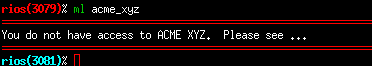
\includegraphics[width=.9\textwidth]{color_banner.png}}
\end{frame}


% page 14
\begin{frame}{Future Work}
  \begin{itemize}
    \item Lmod can optionally track usage.
    \item Future: Make it easier to not remember loads after 1 year.
    \item Get Lmod to support the break function.
    \item Support for Tmod4's advanced version specifiers
      \texttt{module load foo@2.4:2.8}
    \item A monthly discussion group?
  \end{itemize}
\end{frame}


% page 15
\begin{frame}[fragile]
    \frametitle{Lmod Doc usage by Country}
    \center{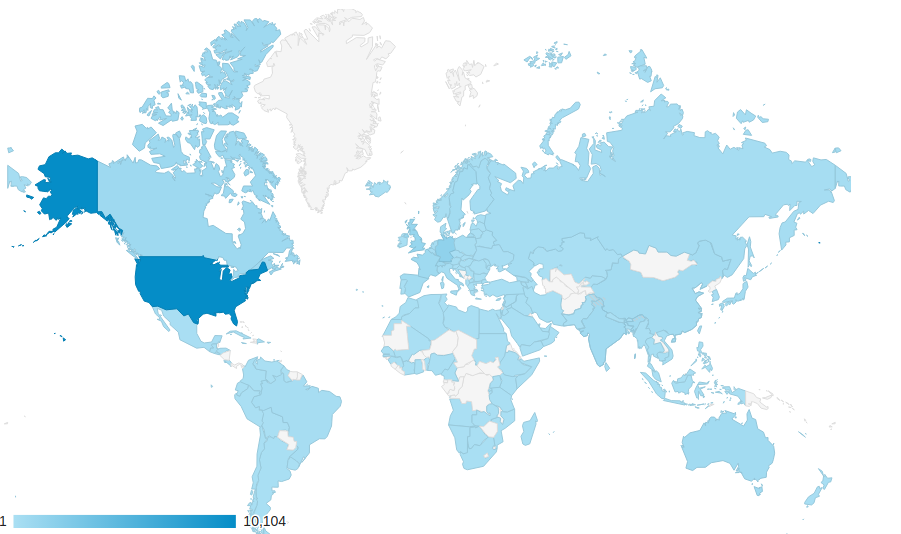
\includegraphics[width=.9\textwidth]{Lmod_usage_by_country}}
\end{frame}

% page 16
\begin{frame}[fragile]
    \frametitle{Lmod Doc usage by City}
    \center{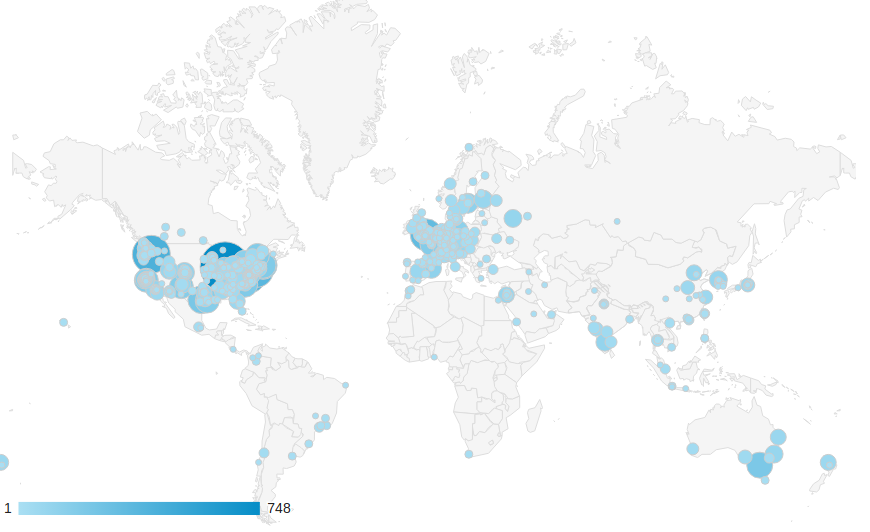
\includegraphics[width=.9\textwidth]{Lmod_usage_by_city}}
\end{frame}

% page 17
\begin{frame}{Conclusions: Lmod 8+}
  \center{\includegraphics[width=.9\textwidth]{Lmod-4color@2x.png}}
  \begin{itemize}
    \item Latest version: https://github.com:TACC/lmod.git
    \item Stable version: http://lmod.sf.net
    \item Documentation:  http://lmod.readthedocs.org
  \end{itemize}
\end{frame}

\end{document}
